\section{Simulation}
\paragraph{6.}
\begin{figure}[H]
\label{fig:sim1}
\begin{center}
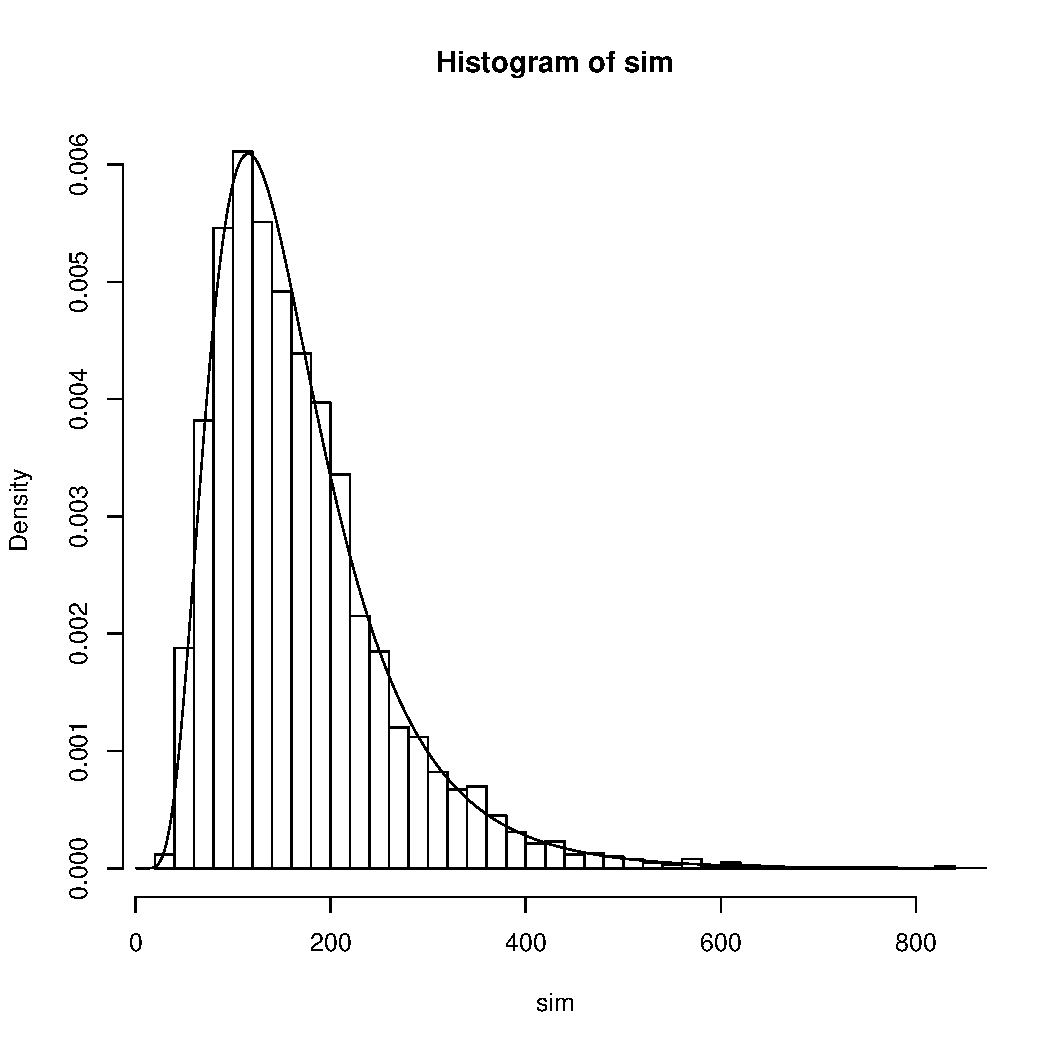
\includegraphics[width=10cm]{graphs/simulation_1.pdf}
\caption{Histogram for de observerede data samt tæthedsfunktionen for
den logaritmiske normalfordeling}
\end{center}
\end{figure}
Histogrammet og tæthedsfunktionen ligner hinanden. Det tyder på at de
observerede data er logaritmisk normalfordelte.
\paragraph{7.}
Stikprøverne stemmer nogenlunde overens med de beregnede resultater.
\begin{figure}[H]
\label{fig:sim2}
\begin{center}
\begin{verbatim}
> c(mean(sim),var(sim),sd(sim),median(sim))
[1]  168.25094 7657.62393   87.50785  149.82703
\end{verbatim}
\caption{}
\end{center}
\end{figure}

\begin{tabular}{c|c|c}
& Stikprøve & Udregning \\
\hline
Gennemsnit & $168,251$ & $168,174$ \\
Varians & $7657,624$ & $8032,96$ \\
Spredning & $87,51$ & $89,63$ \\
Median & $149,827$ & $148,413$ \\
\end{tabular}

